
%(BEGIN_QUESTION)
% Copyright 2013, Tony R. Kuphaldt, released under the Creative Commons Attribution License (v 1.0)
% This means you may do almost anything with this work of mine, so long as you give me proper credit

A helpful strategy for qualitatively analyzing control systems is to mark the inputs of all loop controller bubbles with either ``+'' or ``$-$'' labels to denote the direction of each controller's action.  This is the same symbology used to mark the inputs of an operational amplifier, where ``+'' represents the noninverting input and ``$-$'' represents the inverting input.  The following illustration shows how the ``+'' and ``$-$'' inputs of an opamp relate to the characteristic equations for direct- and reverse-acting proportional controllers:

$$\includegraphics[width=15.5cm]{i04555x03.eps}$$

One way to get yourself into this mind-set of marking loop controller inputs with ``+'' and ``$-$'' symbols is to completely replace the ISA-standard ``bubble'' symbols with triangular opamp symbols.  Try doing this in the following PFD, showing the proper direction of action for each controller for the maple syrup evaporator process by the proper orientation of the opamp symbols' inverting and noninverting inputs (PV versus SP):

$$\includegraphics[width=15.5cm]{i04555x01.eps}$$

\underbar{file i04555}
%(END_QUESTION)





%(BEGIN_ANSWER)

$$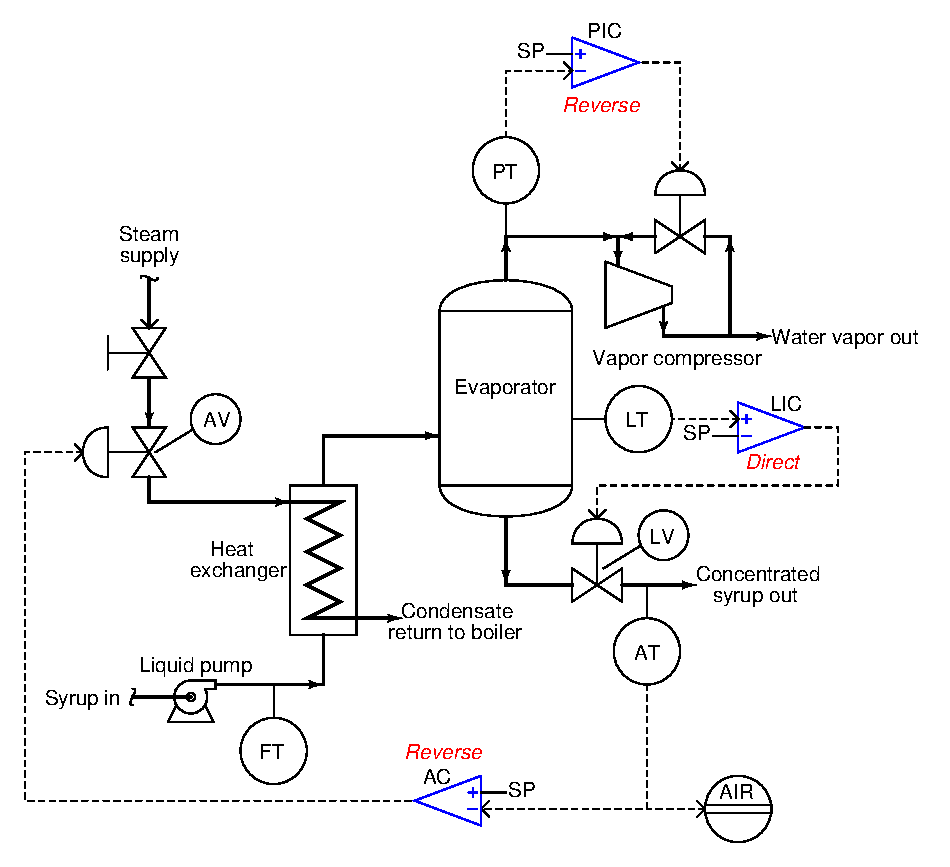
\includegraphics[width=15.5cm]{i04555x02.eps}$$

The analytical controller (AC) is reverse-acting in order to close off the steam valve if the sugar concentration of the syrup increases.

\vskip 10pt

The level indicating controller (LIC) is direct-acting in order to open up the discharge valve if the evaporator level increases.

\vskip 10pt

The pressure indicating controller (PIC) is reverse-acting in order to open up the compressor recycle valve if the pressure inside the evaporator decreases (i.e. if the vacuum becomes too strong).

%(END_ANSWER)





%(BEGIN_NOTES)


%INDEX% Basics, control: direct versus reverse controller action
%INDEX% Process: maple syrup concentration (single-effect evaporator)

%(END_NOTES)


